\chapter{\IfLanguageName{dutch}{Stand van zaken}{State of the art}}%
\label{ch:stand-van-zaken}

% Tip: Begin elk hoofdstuk met een paragraaf inleiding die beschrijft hoe
% dit hoofdstuk past binnen het geheel van de bachelorproef. Geef in het
% bijzonder aan wat de link is met het vorige en volgende hoofdstuk.

% Pas na deze inleidende paragraaf komt de eerste sectiehoofding.

Dit hoofdstuk bevat je literatuurstudie. 
De inhoud gaat verder op de inleiding, maar zal het onderwerp van de bachelorproef *diepgaand* uitspitten. 
De bedoeling is dat de lezer na lezing van dit hoofdstuk helemaal op de hoogte is van de huidige stand van zaken (state-of-the-art) 
in het onderzoeksdomein. 
Iemand die niet vertrouwd is met het onderwerp, 
weet nu voldoende om de rest van het verhaal te kunnen volgen, 
zonder dat die er nog andere informatie moet over opzoeken \autocite{Pollefliet2011}.

Je verwijst bij elke bewering die je doet, vakterm die je introduceert, enz.\ naar je bronnen. 
In \LaTeX{} kan dat met het commando \texttt{$\backslash${textcite\{\}}} of \texttt{$\backslash${autocite\{\}}}. 
Als argument van het commando geef je de ``sleutel'' van een ``record'' in een bibliografische databank in het Bib\LaTeX{}-formaat
 (een tekstbestand). Als je expliciet naar de auteur verwijst in de zin (narratieve referentie), 
 gebruik je \texttt{$\backslash${}textcite\{\}}. Soms is de auteursnaam niet expliciet een onderdeel van de zin, 
 dan gebruik je \texttt{$\backslash${}autocite\{\}} (referentie tussen haakjes). Dit gebruik je bv.~bij een citaat, 
 of om in het bijschrift van een overgenomen afbeelding, broncode, tabel, enz. te verwijzen naar de bron. 
 In de volgende paragraaf een voorbeeld van elk.

\textcite{Knuth1998} schreef een van de standaardwerken over sorteer- en zoekalgoritmen. 
Experten zijn het erover eens dat cloud computing een interessante opportuniteit vormen, zowel voor gebruikers als voor dienstverleners op vlak van informatietechnologie~\autocite{Creeger2009}.

Let er ook op: het \texttt{cite}-commando voor de punt, dus binnen de zin. Je verwijst meteen naar een bron in de eerste zin die erop gebaseerd is, 
dus niet pas op het einde van een paragraaf.



Dit hoofdstuk bevat een literatuurstudie die de gebruikten technologieën gaat omschrijven. 
Daarnaast worden ook eerdere studies naar deze technologieën vermeld. 
Ten eerste wordt een precieze beschrijving gegeven over de programmeertaal javascript en hoe deze wordt gebruikt bij de runtime-omgevingen.
Nadien wordt verder ingegaan op 2 van deze omgevingen namelijk Node.js en Bun.

\section{Javascript}
Javascript is een programmeertaal die gebruikt wordt om applicaties te ontwikkelen. 
Specifiek is het een scripting taal die gebruikt om web pagina's interactief te maken~\autocite{Mozilla2023}.
Hierbij spreken we over client-side Javascript. Wanneer een web pagina wordt bekeken zal de javascript code worden 
gedownload en uitgevoerd~\autocite{JonathanBrownCFA2024}. Langs de andere kant heb je ook nog Server-side javascript. 
Hierbij wordt de code uitgevoerd op de server in plaats van op de client~\autocite{JonathanBrownCFA2024}. 
Voor deze code dan te laten uitvoeren is een javascript runtime-omgeving nodig. 

\subsection{Javascript runtime-omgeving}
Een javascript-omgeving bestaat uit alle componenten om javascript correct te laten werken ~\autocite{Christopher}. 
Het bevat een JavaScript engine, WEB APIs en een callback queue ~\autocite{Christopher}. 
Deze runtime zal dan javascript code omzetten in code die verstaanbaar is voor de computer.
De omgeving specificeert waar dit wordt gedaan, dit kan in een browser maar ook in andere omgevingen zoals een server.
Met behulp van javascript runtime-omgevingen zoals Node.js en Bun kan javascript code ook buiten de browser worden uitgevoerd~\autocite{Mozilla2023}.

\subsubsection{Javascript engine, WEB APIs en callback queue}

In een artikel van ~\textcite{Christopher}, 
wordt uitgelegd dat de javascript engine een simpel computer programma is dat de code kan interpreteren en uitvoeren.
Elk browser heeft zijn eigen Javascript engine achterliggend. Het meest bekende hiervan is de
V8 engine die zowel bij Google chrome als Node.js wordt gebruikt. 
Wanneer een stuk code in de engine wordt gestoken zal deze eerst gelezen worden (parsing). 
De code wordt hierbij omgezet in een data structuur genaamd abstract syntax tree (AST).
Wanneer deze boom is aangemaakt zal de compiler deze omzetten naar machine code. 
Eenmaal deze code is gegenereerd zal de engine zogenaamde execution contexts aanmaken om de code uit te voeren.
In figuur ~\ref{fig:javascriptengine} wordt hiervan een visuele voorstelling getoond.
\begin{figure}[H]
    \centering
    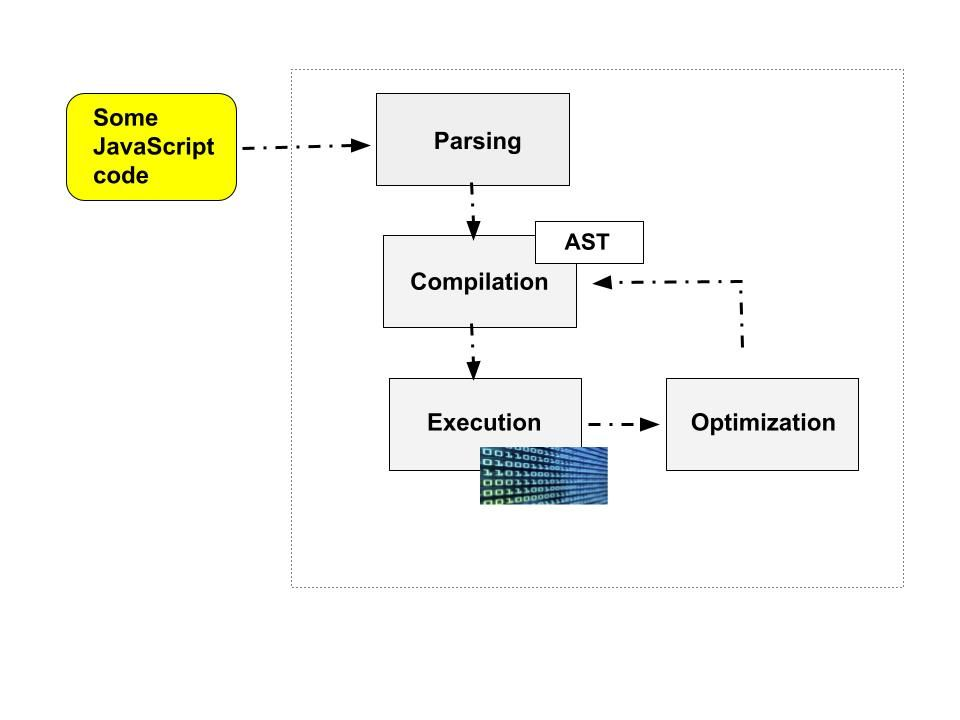
\includegraphics[width=.9\textwidth]{graphics/javascriptengine.jpeg}
    \caption{\label{fig:javascriptengine}}Visuele voorstelling van werking javascript engine ~\autocite{Christopher}.
\end{figure}

Naast een Javascript engine bevat een runtime-omgeving ook WEB APIs en een callback queue. 
WEB APIs zijn functionaliteiten die specifiek voor de runtime omgeving zijn en dus geen deel uitmaken van de javascript taal.
De callback queue zorgt ervoor dat callback functions volgens de First-In-First-Out methode worden uitgevoerd.

\section{Node.js}
De afgelopen jaren is het aantal runtime-omgevingen sterk toegenomen. De meest bekende en oudste hiervan is Node.js.
Node.js is een server-side framework dat wordt gebruikt voor schaalbare applicaties te maken ~\autocite{Gackenheimer2013}.
Het maakt gebruik van de javascript V8 engine ontwikkeld door Google en heeft zijn eigen package manager genaamd Node Package Manager (npm).

\subsection{Event loop}
In het boek van ~\textcite{Ali2013} wordt verteld hoe Node.js zich onderscheidt van andere platformen door het gebruik van een event loop.
Wanneer in Node.js data wordt gelezen of geschreven zal een gebeurtenis worden uitgezonden. 
Aan de hand van zelfgedefinieerde callbacks, verwijzingen naar uitvoerbare code, kan gereageerd worden op deze gebeurtenissen. 
De event loop zal hierbij continu kijken of er gebeurtenissen voorkomen, en wanneer dit zo is zal het deze in de event wachtrij plaatsen.
De event loop zal dan deze wachtrij doorgaan en één per één de event handlers uitvoeren. 
Dit laat toe om I/O operaties asynchroon te maken zonder hierbij multithreading te gebruiken.
In figuur ~\ref{fig:eventloop} wordt hiervan een visuele voorstelling getoond.
\begin{figure}[h]
    \centering
    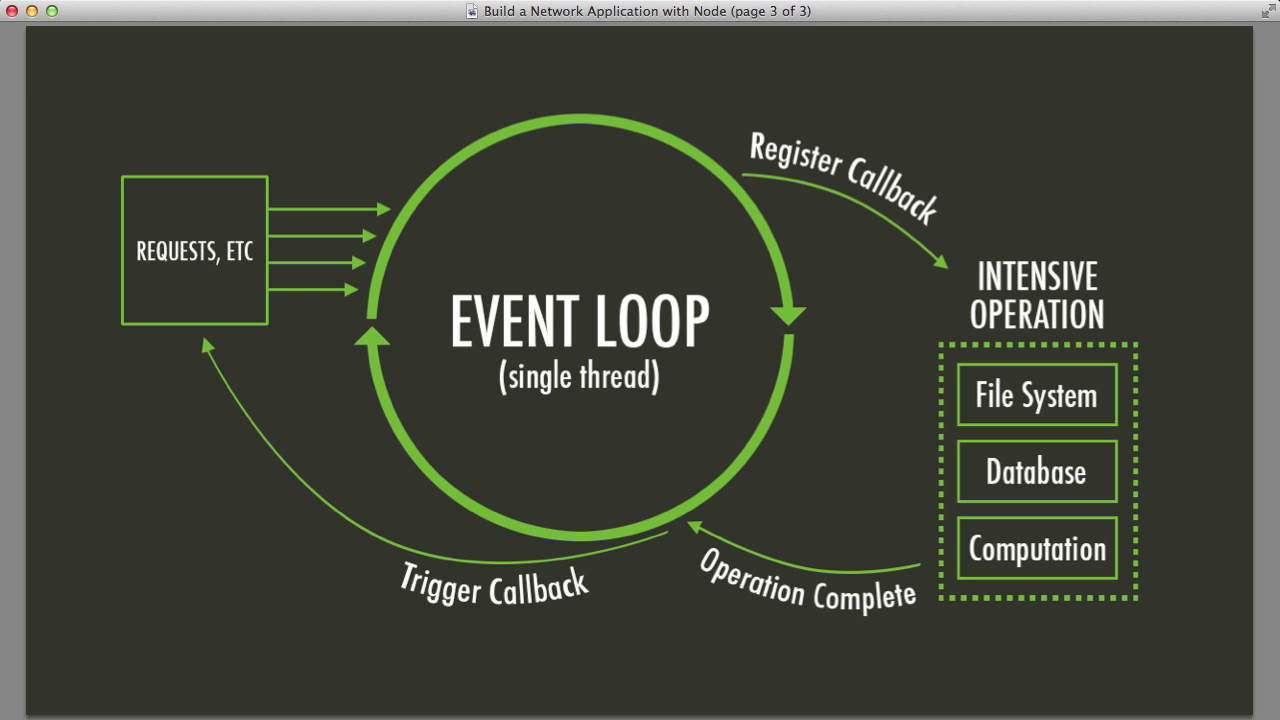
\includegraphics[width=.9\textwidth]{graphics/eventloop.png}
    \caption{\label{fig:eventloop}}Visuele voorstelling van de event loop ~\autocite{Luxembourg2023}.
\end{figure}

\subsection{Node Package Manager}
Node.js maakt gebruik van modules om code te hergebruiken. 
Zo vormt een module een stuk herbruikbare javascript code 
die je kan importeren in een ander javascript bestand ~\autocite{Semah2022}.
Naast deze zelf te maken kan je ook modules of packages van andere ontwikkelaars gebruiken met behulp van de Node Package Manager.
Veel van deze packages hangen af van nog andere packages om correct te werken \autocite{kula2017}.
Aan de hand van een package.json bestand kunnen packages toegevoegd worden aan een project.
\begin{figure}[h!]
    \centering
    \begin{minted}[bgcolor=bg,
        fontfamily=tt,
        linenos=true,
        numberblanklines=true,
        numbersep=5pt,
        gobble=0,
        framesep=2mm,
        tabsize=4,
        obeytabs=false,
        breaklines=true,
        mathescape=false
        samepage=false,
        showspaces=false,
        showtabs =false,
        texcl=false]{js}
        {
          "dependencies": {
            "foo": "1.0.0 - 2.9999.9999",
            "bar": ">=1.0.2 <2.1.2",
            "baz": ">1.0.2 <=2.3.4",
            "boo": "2.0.1",
            "qux": "<1.0.0 || >=2.3.1 <2.4.5 || >=2.5.2 <3.0.0",
            "asd": "http://asdf.com/asdf.tar.gz",
            "til": "~1.2",
            "elf": "~1.2.3",
            "two": "2.x",
            "thr": "3.3.x",
            "lat": "latest",
            "dyl": "file:../dyl"
            }
        }
        \end{minted}
        \caption{Voorbeeld package.json \autocite{Kaplan2024}}
\end{figure}

\section{Bun}
Performantie is één van de belangrijkste zaken bij een server-side framework. 
Daarom is Node.js dankzij zijn event-gedreven I/O model een veelvoorkomende keuze als het gaat om server-side frameworks.
Echter wil Bun dit veranderen door nog meer focus te leggen op snelheid en performantie.

\subsection{JavascriptCore}
Eén van de manieren waardoor Bun dit bereikt is door het gebruiken van een andere Javascript engine.
Bun gebruikt JavaScriptCore in plaats van de V8 Javascript engine die Node.js gebruikt. 
Deze zou volgens ~\textcite{McDonnel2023} ervoor zorgen dat Bun 4 keer sneller opstart dan Node.js. 
De engine is ingebouwd in WebKit, een web browser engine die wordt gebruikt binnen het Apple ecosysteem voor macOS en IOS.
In een artikel van ~\textcite{Pizlo2020} wordt uitgelegd dat bij de executie een script door verschillende fases gaat:
\begin{itemize}
    \item De lexer is verantwoordelijking voor het opbreken van het script in een reeks tokens.
    \item De parser gaat deze tokens gebruiken om een een asbract syntax tree te maken.
    \item De Low-Level Interpreter (LLINT) zal bytecode produceren dat JavaScriptCore kan uitvoeren.
\end{itemize}
Daarnaast zijn er hierbij ook nog optimalisaties voor instructies die vaak terugkeren. 
JavascriptCore zal instructies in 4 verschillende lagen uitvoeren, afhankelijk van hoeveel keer ze worden uitgevoerd:
\begin{enumerate}
    \item De Low-Level Interpreter (LLINT) zal zoals hierboven beschreven instructies omzetten in bytecode.
    \item De baseline JIT zal een stuk code at runtime uitvoeren in plaats van ervoor. 
    Hierbij worden de bytecode operaties omgezet naar een template van machine code zonder veel optimalisaties. Deze laag is snel.
    \item De Data Flow Graph JIT zal een data-flow graaf gebruiken van de code om zo complexe optimalisaties uit te voeren die betrekking hebben tot de stroom van de code.
    \item De Faster than Light JIT zal nog meer optimalisaties toevoegen bovenop de optimalisaties van de Data Flowh Graph JIT. 
    Deze laag is duurder en wordt enkel gebruikt voor code die kunnen profiteren van optimalisaties.
\end{enumerate}
Via de Low-Level Interpreter zal een profile voor elke instructie aangemaakt worden. 
Aan de hand hiervan weet de engine hoeveel keer een instructie wordt uitgevoerd en in welk niveau ze zitten.
LLINT zorgt ervoor dat het geheugengebruik wordt gereduceerd. Zo kost het genereren van machine code zeer veel geheugen.
Doormiddel van LLINT moeten we niet voor alle javascript code de bijhorende machine code genereren.